\documentclass{article}

\usepackage{fancyhdr}
\usepackage{extramarks}
\usepackage{amsmath}
\usepackage{amsthm}
\usepackage{amsfonts}
\usepackage{tikz}
\usepackage[plain]{algorithm}
\usepackage{algpseudocode}
\usepackage{xepersian}
 \renewcommand{\refname}{\rl{{مراجع}\hfill}}
\settextfont[Scale=1.2]{XB Niloofar}
%\setlatintextfont{Serif}
\setdigitfont[Scale=1.2]{Yas}
\DefaultMathsDigits


\usetikzlibrary{automata,positioning}

%
% Basic Document Settings
%

\topmargin=-0.35in
\evensidemargin=0in
\oddsidemargin=0in
\textwidth=6.5in
\textheight=9.0in
\headsep=0.25in

\linespread{1.1}

\pagestyle{fancy}
\lhead{بهراد منیری}
\rhead{جداسازی کور ترکیب‌های غیرخطی فرآیند‌های تصادفی}
\lfoot{\lastxmark}
\cfoot{\thepage}

\renewcommand\headrulewidth{0.4pt}
\renewcommand\footrulewidth{0.4pt}

\setlength\parindent{0pt}

\title{جداسازی کور ترکیب‌های غیرخطی فرآیند‌های تصادفی}
\author{
	بهراد منیری\\
	\texttt{bemoniri@ee.sharif.edu}\\
	\normalsize{دانشکده‌ی مهندسی برق، دانشگاه صنعتی شریف، آزادی، تهران، ایران}
	\vspace{0.5cm}\\
	استاد راهنما:
	دکتر مسعود بابائی‌زاده
}
\date{}

\renewcommand{\part}[1]{\textbf{\large Part \Alph{partCounter}}\stepcounter{partCounter}\\}

%
% Various Helper Commands
%

% Useful for algorithms
\newcommand{\alg}[1]{\textsc{\bfseries \footnotesize #1}}


\newtheorem{den}{{\large\bf تعریف}}[section]
\newtheorem{exa}{{\large\bf مثال}}[section]
\newtheorem{lem}{{\large\bf لم}}[section]
\newtheorem{pro}{{\large\bf گزاره}}[section]
\newtheorem{cor}{{\large\bf نتیجه}}[section]
\newtheorem{thm}{{\large\bf قضیه}}[section]
\newtheorem{rem}{{\large\bf تذکر}}[section]
\newtheorem{nnt}{{\large\bf توجه}}[section]
\newtheorem{aaa}{{\large\bf}}[section]

\begin{document}
\maketitle
در این پروژه، به بررسی مسئله‌ی جداسازی کور ترکیب‌های غیر‌خطی می‌پردازیم. این مسئله،  عموماً به عنوان یکی از مهم‌ترین مسائل باز در حوزه‌ی یادگیری ماشین نظارت‌نشده تلقی می‌شود
\cite{hyvarinen2017nonlinear}.
فرض کنید که فرآیند‌های تصادفی‌ مستقل
$\textbf{s}(t) = [s_1(t), s_2(t), \dots, s_n(t)]^\top$،
 وجود داشته باشند که مشاهده نشده‌اند.  سیگنال‌های
$[x_1(t), x_2(t), \dots x_n(t)]^\top = f\Big([s_1(t), s_2(t), \dots s_n(t)]^\top\Big)$
که در آن، تابع 
$f: \mathbb{R}^n \to \mathbb{R}^n$،
یک تابع ناشناخته است، مشاهده شده‌اند. هدف اصلی مسئله‌ی جداسازی کور منابع، یافتن تابع $f$ و همچنین سیگنال‌های 
$\textbf{s}(t) = [s_1(t), s_2(t), \dots, s_n(t)]^T$
بر اساس مشاهدات ما از سیگنال‌های 
$[x_1(t), x_2(t), \dots, x_n(t)]^T$
است.

در صورتی که فرآیند‌های تصادفی
$\textbf{s}(t)$
در زمان، وابستگی نداشته باشند، یعنی سفید باشند، می‌توان مثال‌‌های فراوانی از توابع $f$ یافت که این فرآیند‌های مستقل را، به فرآیند‌های مستقل تبدیل کند. تا مدت‌ها تصوّر بر این بوده است که اعمال شرط هموار بودن بر تابع 
$f$
جواب این مسئله را یکتا می‌کند، اما در سال 2002، دکتر بابائی زاده مثالی از تابعی هموار ارائه‌ دادند که قادر بود فرآیند‌های سفید را به فرآیند‌های سفید تبدیل کند. این مثال نشان می‌دهد که در حالتی که فرآیند‌های تصادفی سفید هستند، جداسازی کور منابع غیرخطی مبتنی بر استقلال منابع ممکن نیست
\cite{mbzadehthesis}.

در سال ۲۰۰۳،
\cite{harmeling2003kernel}
ایده‌ی استفاده از وابستگی‌های زمانی را برای جداسازی ترکیب‌های غیرخطی فرآیند‌های تصادفی مطرح کردند. در این مقاله‌ الگوریتمی برای جداسازی ترکیب‌های غیرخطی، با استفاده از روابط زمانی ارائه شده است که علی‌رغم عملکرد تجربی بسیار امیدوارکننده‌ی آن، اثباتی برای صحت عملکرد آن ارائه نمی‌کرد.

در سال ۲۰۱۷، در مقاله‌ی
\cite{hyvarinen2017nonlinear}
قضیه‌ای برای جدایی‌پذیری ترکیب‌های غیرخطی فرآیند‌های تصادفی ارائه‌ شده‌است که در ادامه به بیان این قضیه می‌پردازیم.
\begin{den}
	دو متغیر تصادفی، 
	\textbf{	به صورت همگن مستقل}
	گفته می‌شوند، اگر
	$$q(x, y) = \frac{\partial^2 \log(p(x, y))}{\partial x \partial y}  \neq 0 \;\;\;\; \forall (x, y)$$
\end{den}
\begin{den}
	یک فرآیند تصادفی $s(t)$،
\textbf{	به صورت همگن مستقل}
		گفته می‌شود، اگر برای هر زمان $t$ دلخواه،
		$s(t)$
		و 
		$s(t-1)$
متغیر های تصادفی
	\textbf{	به صورت همگن مستقل}
	باشند.
\end{den}
\begin{den}
یک فرآیند‌ تصادفی، شبه-گاوسی گفته می‌شود، اگر برای هر زمان $t$ آن داشته باشیم:
$$\frac{\partial^2 \log(p(x(t), x(t-1))}{\partial x(t)\partial x(t-1)} = c\alpha\Big(x(t)\Big)\alpha\Big(x(t-1)\Big)$$
که $\alpha$  تابعی دلخواه  وآلفا، یک عدد دلخواه است.
\end{den}

\begin{thm}
اگر فرآیند‌های تصادفی
$s_i(t)$
مشترکاً مستقل، ایسان به معنای سخت‌گیرانه و ارگودیک  و به صورت همگن مستقل باشند و  هیچ یک از آن‌ها شبه‌گوسی نباشد. با فرض اینکه تابع $f$ وارون‌پذیر بوده و خودش و وارون آن دو بار مشتق‌پذیر با مشتق پیوسته باشند، با مشاهده‌ی فرآیند‌های تصادفی
 $x_i(t)$،
 تابع $f$ و همچنین فرآیند‌‌های تصادفی مستقل $s_i(t)$ به صورت یکتا قابل بازیابی هستند.
\end{thm}
اثبات این مقاله‌ برای قضیه‌ی فوق، اثباتی ساختنی است و الگوریتمی ارائه می‌کند که جداسازی را انجام دهد.

بعد از بررسی دقیق اثبات مقاله‌ی فوق توسط من، مشخص شد که در اثبات آن مقاله ایرادی وجود دارد. یکی ازاهداف اصل من در این پروژه، اصلاح این اثبات است.

این قضیه، شرایطی بسیار سخت‌گیرانه بر روی فرآیند‌های تصادفی قرار می‌دهد و تا کنون مشخص نیست که این شرایط، تا چه اندازه می‌توانند محدود‌کننده باشند. یکی از اهداف این پروژه، یافتن دسته‌ای از فرآیند‌های تصادفی با شرایط فوق و بررسی میزان محدودیت اعمال شده توسط آن شرایط است.

الگوریتم یادگیری مطرح شده در این مقاله نیز الگوریتمی است که از نظر محاسباتی، بهینه نیست و دومین هدف من در این پروژه، ارائه الگوریتمی کارا برای انجام این جداسازی است. ایده‌ی ما برای طراحی الگوریتم، یافتن تابع $g$  است، به نحوی که
 $\textbf{y}(t) = g(\textbf{x}(t)) = gof(\textbf{x}(t))$
 فرآیند‌هایی تصافی با کمترین اطلاعات متقابل ممکن باشند. ایده‌ای مشابه در سال ۲۰۰۵ در مقاله‌ی 
 \cite{babaie2005general}
 مطرح شده است که قصد داریم در این پروژه، از ایده‌هایی مشابه با آن استفاده کنیم.
 
جداسازی کور منابع، کاربرد‌های فراوانی دارد. به عنوان مثال، در هنگام اسکن برگه‌های نازک، بسیار رایج است که سایه‌ای از پشت یک صفحه‌، در اسکن آن ظاهر شود (شکل 
\ref{pages}).
 جداسازی کور منابع، می‌تواند برای جداسازی نوشته‌های هر دو صفحه‌، با مشاهده‌ی اسکن هر دو سمت برگه به کار رود. این ترکیب به شدت غیر خطی است
\cite{comon2010handbook}
و این روش جدید می‌تواند برای جداسازی  چنین ترکیب‌هایی موثر باشد.
 
\begin{figure}[h!]
	\centering
	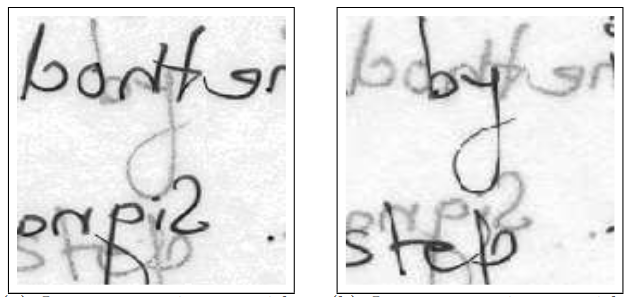
\includegraphics[scale=0.4]{application1.png}
	\caption{یکی از کاربرد‌های احتمالی جداسازی کور منابع، برای تفکیک نوشته‌های صفحات مختلف در اسکن}
	\label{pages}
\end{figure}

\begin{latin}
		\bibliographystyle{acm}
		\bibliography{bib}
\end{latin}

\pagebreak


\end{document}
